\documentclass[reportComp]{thesis}
\usepackage[cpp,pseudo]{mypackage}

\title{模式识别作业三}
\subtitle{上机练习}
\school{数据科学与计算机学院}
\author{陈鸿峥}
\classname{17大数据与人工智能}
\stunum{17341015}
\headercontext{模式识别作业}
\lstset{language=python}

\begin{document}

\maketitle

\begin{question}[\textsection 2.5 Q1]
下面的几道题可能会用到如下的程序:
\begin{itemize}
	\item [(a)] 写一个程序产生服从$d$维正态分布$N(\vmu,\Sigma)$的随机样本
	\item [(b)] 写一个程序计算一给定正态分布及先验概率$P(\omega_i)$的判别函数(式(49)中所给的形式)。
	\item [(c)] 写一个程序计算任意两个点间的欧式距离。
	\item [(d)] 在给定协方差矩阵$\Sigma$的情况条件下,写一个程序计算任意一点$\vx$到均值$\vmu$间的Mahalanobis距离。
\end{itemize}
\end{question}
% https://math.stackexchange.com/questions/2079137/generating-multivariate-normal-samples-why-cholesky

\section{实验过程及代码}
原理分析如下
\begin{itemize}
	\item [(a)] $d$维多元正态密度的形式如下
	\[p(\vx)=\frac{1}{(2\pi)^{d/2}|\Sigma|^{1/2}}\exp\lrs{-\frac{1}{2}(\vx-\vmu)^\T\Sigma^{-1}(\vx-\vmu)}\]
	对$\Sigma$进行乔列斯基分解,得到$\Sigma=L L^\T$,故随机样本为$L\vv+\vmu$,其中$\vv$为$d$维的随机数,用以表示偏移量。
	\item [(b)] 正态分布的判别函数为
	\[g(\vx)=-\frac{1}{2}(\vx-\vmu)^\T\Sigma^{-1}(\vx-\vmu)-\frac{d}{2}\ln 2\pi-\frac{1}{2}\ln|\Sigma|+\ln P(\omega)\]
	\item [(c)] 即求两个点$\vv_1$和$\vv_2$的L2范数。
	\item [(d)] 由Mahalanbois距离的定义
	\[d_M^2=(\vx-\vmu)^\T\Sigma^{-1}(\vx-\vmu)\]
\end{itemize}

程序如下,采用Python进行编写,并且利用numpy包进行矩阵运算。
有些是numpy中有现成函数,但我也写了两个版本互相进行验证(一种基于基本的矩阵运算,一种直接使用numpy封装好的包)。
\begin{lstlisting}
import numpy as np

def normal_distribution(mu,sigma,size=10):
	"""
	Generate d-dimensional normal distribution N(mu,Sigma)
	mu: d-dim vector
	Sigma: d*d-dim covariance matrix
	n: number of generated points
	"""
	# return np.random.multivariate_normal(mu,sigma,size)
	return np.dot(np.random.randn(size,mu.size), np.linalg.cholesky(sigma)) + mu

def discriminant(x,mu,sigma,p_omega):
	"""
	g(x) = ln p(x|omega) + ln P(omega)
	"""
	d = mu.size
	return -1/2 * Manhalanobis(x,mu,sigma) - d/2 * np.log(np.pi) - 1/2 * np.log(np.abs(np.linalg.det(sigma))) + np.log(p_omega)

def L2(p1,p2):
	"""
	Euclidean distance (L2 distance)
	"""
	# return np.linalg.norm(p1-p2)
	return np.sqrt(np.sum(np.power(p1-p2,2)))

def Manhalanobis(x,mu,sigma):
	"""
	Given covariance matrix Sigma, compute the Manhalanobis distance
	from point x to mean mu
	"""
	return (x-mu).T.dot(np.linalg.inv(sigma)).dot((x-mu))
\end{lstlisting}

并且编写了一组测试样例进行检验
\begin{lstlisting}
m = np.random.rand(4,10)
mu = np.mean(m,axis=1)
sig = np.cov(m)
v1 = m.T[1]
v2 = m.T[2]
print(normal_distribution(mu,sig))
print(discriminant(v1,mu,sig,1/2))
print(L2(v1,v2))
print(Manhalanobis(v1,mu,sig))
\end{lstlisting}

\section{实验结果与分析}
结果如下图所示。
\begin{figure}[H]
\centering
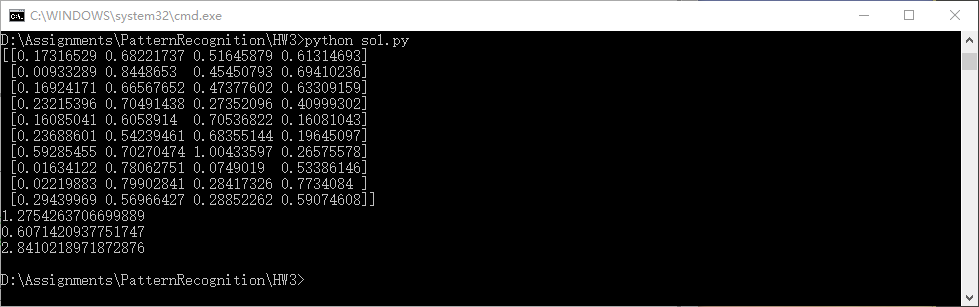
\includegraphics[width=\linewidth]{result.png}
\end{figure}
可以看到程序正常生成了10个4维的随机数,同时以\verb'v1'和\verb'v2'作为输入样例,计算了判别函数、欧式距离和Manhalanobis距离,结果均正常显示并且验证正确。

\section{实验总结}
本次实验主要将贝叶斯决策论的一些基本函数给实现了,由于基于Python的矩阵运算库numpy,因此整个实现过程还是相对比较简单的。


\end{document}
% ftp://222.200.180.156/
% student
% 2019s
% 实验作业次数_学号_姓名

% 如何用python numpy产生一个正态分布随机数的向量或者矩阵? - 采石工的回答 - 知乎
% https://www.zhihu.com/question/39823283/answer/115241445